\documentclass[../m082main.tex]{subfiles}
\graphicspath{{\subfix{../figures/}}}

\begin{document}

\chapter{First-Order Differential Equations}

\section{Separable Differential Equations}
The first class of differential equations we'll discuss involves those first-order differential equations that can, broadly, be "separated" into its independent and dependent variables.

\begin{definition}[Separable differential equation]
    An ordinary differential equation is separable if it can be written in the form
    \[ \frac{dy}{dt} = G(y) \cdot H(t). \]
\end{definition}

\begin{example}[Solving a separable ODE]
    Suppose we are given the separable ODE
    \begin{align}
        \frac{dy}{dt} &= G(y) \cdot H(t). \\
        \intertext{To solve this differential equation, we begin by moving the $y$-dependent stuff to the left side:}
        \frac{1}{G(y)} \cdot \frac{dy}{dt} &= H(t). \\
        \intertext{Now we integrate both sides with respect to $t$:}
        \int \frac{1}{G(y)} \cdot \frac{dy}{dt} \;dt &= \int H(t) \;dt \\
        \intertext{For the integral on the left we can do a change of variabes from $t$ to $y$ to get}
        \int \frac{dy}{G(y)} &= \int H(t) \;dt.
    \end{align}
    From here, all that's left to do is make the resulting equation as simple as possible.
    This may or may not involve solving for $y$, depending on how complex the solution is.

    \medskip
    \textit{Note: In practice, we normally skip from Equation (2.1) directly to Equation (2.4).
    I only included some extra steps here to show why we can sort of treat the $dy/dt$ as a fraction and move the $dt$ to the right side of the equation.}
\end{example}

\section{First-Order Linear Differential Equations}
Here, we provide a way to solve any first-order linear differential equation.
Though this method will be less obvious than separation of variables, what will be more obvious is when we can actually apply the method.

\begin{example}[Solving a first-order linear ODE]
    All first-order linear ODEs can be written in the form
    \[ a(x)y' + b(x)y = c(x). \]
    However, this DE will be more useful to us when it is in normal form:
    \begin{align*}
        y' + p(x)y &= q(x) \\
        \intertext{We multiply by some function $\mu(x)$ that satisfies $\mu'(x) = \mu(x)p(x)$:}
        \mu(x)y' + \mu(x)p(x)y &= \mu(x)q(x) \\
        \mu(x)y' + \mu'(x)y &= \mu(x)q(x) \\
        \intertext{By the product rule,}
        \frac{d}{dx} \left[ \mu(x) \cdot y \right] &= \mu(x)q(x) \\
        \intertext{Integrating with respect to $x$:}
        \mu(x) \cdot y &= \int \mu(x)q(x) \;dx \\
        y &= \frac{1}{\mu(x)} \int \mu(x)q(x) \;dx
    \end{align*}
    This gives an explicit solution to the DE.
    But what is the function $\mu(x)$?
    Recall that we have the separable DE
    \[ \frac{d\mu}{dx} = \mu(x)p(x). \]
    The solution to this DE turns out to be
    \[ \mu(x) = e^{\int p(x) \;dx}. \]
    For this reason, $\mu(x)$ is called the integrating factor for first-order linear ODEs. 
\end{example}

We summarize this example with a theorem.

\begin{theorem}[Integrating factor method for solving first-order linear ODEs]
    Suppose we have a first-order linear ODE in its normal form
    \[ y' + p(x)y = q(x). \]
    If we define an integrating factor $\mu(x) = e^{\int p(x) \;dx}$, then the general solution to this DE is
    \[ y = \frac{1}{\mu(x)} \int \mu(x)q(x) \;dx. \]
\end{theorem}

\section{Numerical Methods}
We'll discuss two numerical methods for visualizing and approximating solutions to initial-value problems.
The first of these is below.

\begin{definition}[Slope field]
Consider the first-order differential equation
\[ \frac{dy}{dx} = f(x, y). \]
The slope field of this DE encodes the value of $dy / dx$ at each point $(x, y)$ as line segments that lay tangent to a solution curve $y(x)$ at each point on a grid.
\end{definition}

Slope fields help us visualize the general trend that solutions to a differential equation follow.

\begin{example}[Slope field of a logistic DE]
    The slope field of the logistic DE $dy / dx = y\left( 1 - y / 5 \right)$ is shown below.
    \begin{center}
        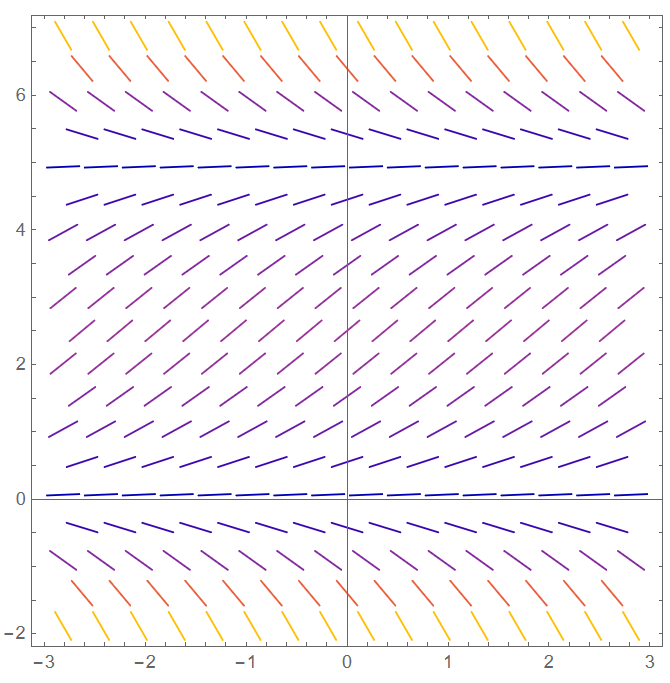
\includegraphics[width=7.5cm]{logisticSlopeField.png}
    \end{center}
    Given a boundary (or in another case, initial) condition $y(x_0) = y_0$, we could use this slope field to sketch a solution curve, using the sloped line segments to "push" the curve in the right direction.
\end{example}

Notice the behavior of the slope field at $y = 0$ and $y = 5$.
At each of these locations we have a series of horizontal line segments.
If a solution curve $y(x)$ ever reaches either of these $y$-values, it will stay there for the rest of its existence because there $dy / dx = 0$.
Despite this similarity, the two "equilibria" are fundamentally different: while solutions tend to converge at $y = 5$, they tend to diverge at $y = 0$.
We summarize these observations below.

\begin{definition}[Equilibrium solution of a first-order DE]
    A solution $y = y(x)$ to a first-order differential equation is called an equilibrium solution to the DE if its derivative $dy / dx = 0$ for all $x$.
    If other solutions tend to converge to an equilibrium, the equilibrium is stable; if other solutions tend to diverge, the equilibrium is unstable.
\end{definition}

Next, we give a way to actually compute approximations for initial-value problems.

\begin{definition}[Euler's method]
    Consider the initial-value problem
    \[ \frac{dy}{dx} = f(x, y), \quad y(x_0) = y_0. \]
    To approximate the value of $y$ at a different $x$-value, we iterate through the following algorithm a sufficient number of times.

    Let $v_0 = y(x_0) = y_0$, and let $\Delta x$ be some small "step."
    Then $v_n$ is an approximation for $y(x_n)$, where
    \begin{align*}
        x_{n+1} &= x_n + \Delta x \\
        v_{n+1} &= v_n + \Delta x \cdot f(x, y)
    \end{align*}
    
\end{definition}

Euler's method is a very bad method for approximating solutions to differential equations.
But it is very simple, based only on a series of tangent line approximations.
Smaller step sizes lead to better approximations.

\section{Existence and Uniqueness of Solutions}
We give two theorems relating to whether or not a sole solution exists for a given DE.
There is a trade-off here: the first theorem gives a stronger result but works on a smaller class of functions.

\begin{theorem}[Existence and uniqueness of solutions to a first-order linear IVP]
    Consider this IVP for a first-order linear DE in normal form:
    \[ y' + p(t)y = q(t) \;\text{ with }\; y(t_0) = y_0. \]
    If the coefficients $p(t)$ and $q(t)$  $(a, b)$ containing $t_0$, then the solution of the IVP exists and is unique on the whole interval $(a, b)$.
\end{theorem}

\begin{theorem}[Existence and uniqueness of solutions to a first-order IVP]
    Consider the IVP for the first-order DE:
    \[ y'(t) = f(t, y) \;\text{ with }\; y(t_0) = y_0. \]
    If $f(t, y)$ and $\frac{\partial f}{\partial y}(t, y)$ are continuous on the rectangle $t \in (\alpha, \beta)$ and $y \in (\gamma, \delta)$ containing $(t_0, y_0)$, then the solution to the IVP exists and is unique on some interval $t \in (t_0 - h, t_0 + h)$ for some $h > 0$.
\end{theorem}

Both of these boil down to the functions in the DE being "well-behaved."
It's reasonable that continuity should be a condition for both of these.
The $\partial f / \partial y$ condition in Theorem 2.3 ensures a smooth transition between two solution curves in the same neighborhood.
In fact, this theorem allows us to state something significant about the solution curves of a DE.

\begin{corollary}[Solution curves do not intersect]
    Under the same hypothesis as Theorem 2.3, two solution curves in the region cannot intersect.
\end{corollary}

\end{document}